\section{State of The Art}
\label{sec:int_state}

Solving the many-body problem remains one of the greatest challenges in physics.
Following the wealth of attempts at such pursuit, certain phenomena arising due to the strong interactions in quantum systems are explained in different theoretical frameworks, namely superconductivity, the Mott metal-insulator transition, and fractional quantum Hall effect.
All of these breakthroughs represented revolutions in their respective fields with significant scientific and technological impact.

Only in very limited cases does an actual analytical solution exist for the  Schr\"odinger equation for a system of interacting particles.
One must resort to sophisticated approximation methods to obtain  information about the role played by the competing interactions under various conditions in the aforementioned cases.
It is then natural that numerical methods have become prominent as a tool for extracting useful information about this type of systems.
\ac{QMC} is amongst the most accurate and extensively studied ones.

The idea of all \ac{QMC} methods is to reduce the interacting problem to solving a set of integrals, which can be evaluated numerically through a standard stochastic procedure.
These integrals are arrived at upon formulating the quantum many-body description of the system using the Schr\"odinger equation.
Hence the name \acl{QMC}, which is used to distinguish it from Classical Monte Carlo.
In the classical version, one measures thermal averages, while in the quantum version, one measures expectations of operators over the Hilbert space of the system, corresponding to physical observables that fluctuate with a dynamics given by the Schr\"odinger equation.

\subsection{Beyond graphene: TMD nanoribbons}

\ac{2D} materials have steadily been attracting more and more attention since graphene was experimentally isolated from a graphite sample by mechanical exfoliation, yielding a system constituted by a single layer of atoms (Figure \ref{fig:graphene}, left).
Since then, numerous studies have been made due to the promising properties of these materials, and the interesting as-yet-unseen phenomena occurring within them, for example: unconventional quantum Hall effect, absence of localization, and electrons behaving like massless relativistic particles (Figure \ref{fig:graphene}, right), providing a bridge between condensed matter physics and quantum electrodynamics \cite{katsnelson_graphene:_2007}.

\begin{figure}[H]
\hspace{1cm}
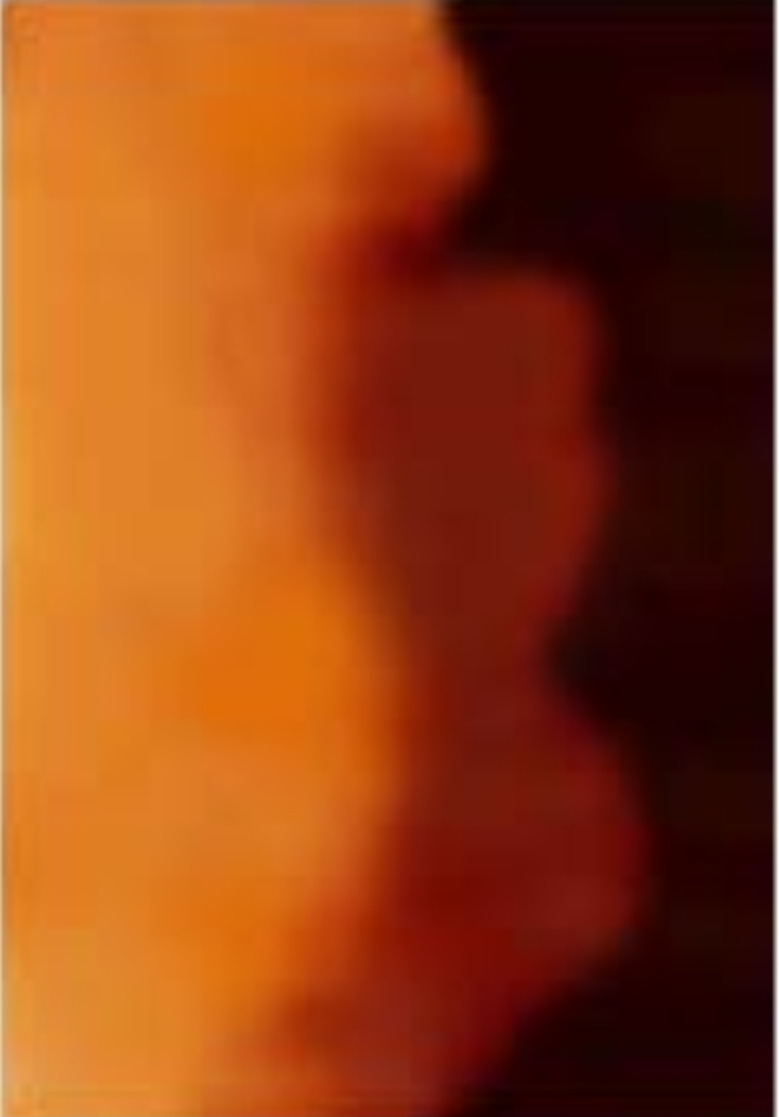
\includegraphics[width = 4.7cm]{Introduction/graphene.png}
\hspace{2cm}
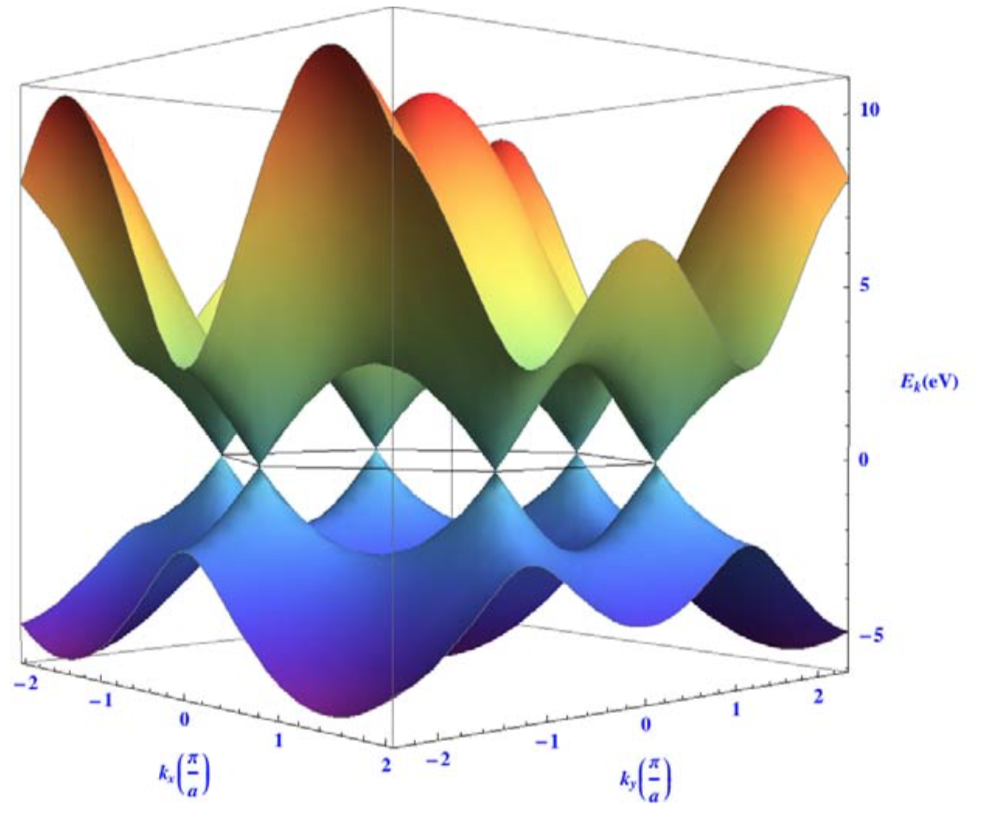
\includegraphics[width = 8.5cm]{Introduction/disp_rel.png}
\caption[Graphene monolayer; graphene's dispersion relation.]{Left: \acf{AFM} picture of a graphene monolayer. The black area is a substrate used for fabrication purposes. The dark orange area is a monolayer of graphene. Right: Dispersion relation of graphene. The black line represents the Fermi energy. Close to it, the dispersion relation is linear, corresponding to massless excitations (taken from \cite{noauthor_nobel_nodate}). }
\label{fig:graphene}
\end{figure}	

On the other hand, \acp{TMD} are a recent member of the \ac{2D} materials family \cite{wang_electronics_2012, roldan_electronic_2014, xu_spin_2014}.
\acp{TMD} have been attracting interest because they seem to overcome some of the drawbacks of graphene in technological applications.
For example, monolayer graphene is gapless, while its bilayer counterpart has only a tunable, but small gap of the order of a tenth of an $eV$.
Contrastingly, \acp{TMD} have an intrinsic gap in excess of $1 \, eV$, being more promising in designing, for example, transistors.
Hole-doped \acp{TMD} are expected to show topological superconductivity \cite{hsu_topological_2017}, while the superconducting phase of graphene has been predicted, but is not easily attained.
Superconductivity in graphene-like \ac{2D} materials is important because it could boost high speed nanoelectronics.
Moreover, the presence of transition metal atoms in \acp{TMD} suggests the possibility of magnetic ordering \cite{braz_valley_2017}, which could be very relevant in nanospintronics applications.
Both topological superconductivity and magnetic ordering arise due to the effect of strong electron correlations.
Thus, to investigate these properties of \acp{TMD} when performing simulations, we need a computational method that is robust enough to capture the effects of electron interactions.

A nanoribbon consists of a \ac{2D} layer that can be regarded as infinitely long on one direction, but not on the other (Figure \ref{fig:fabrication}), so that edge states become relevant, and can be controlled to yield interesting properties.
For simulation purposes, it is natural to assume translational invariance along the ribbon's longitudinal direction, and use \acp{PBC}.
On the other direction, we use \acp{OBC}, effectively considering zigzag edges (Figure \ref{fig:nanoribbons}, left).

\begin{figure}[H]
\centering
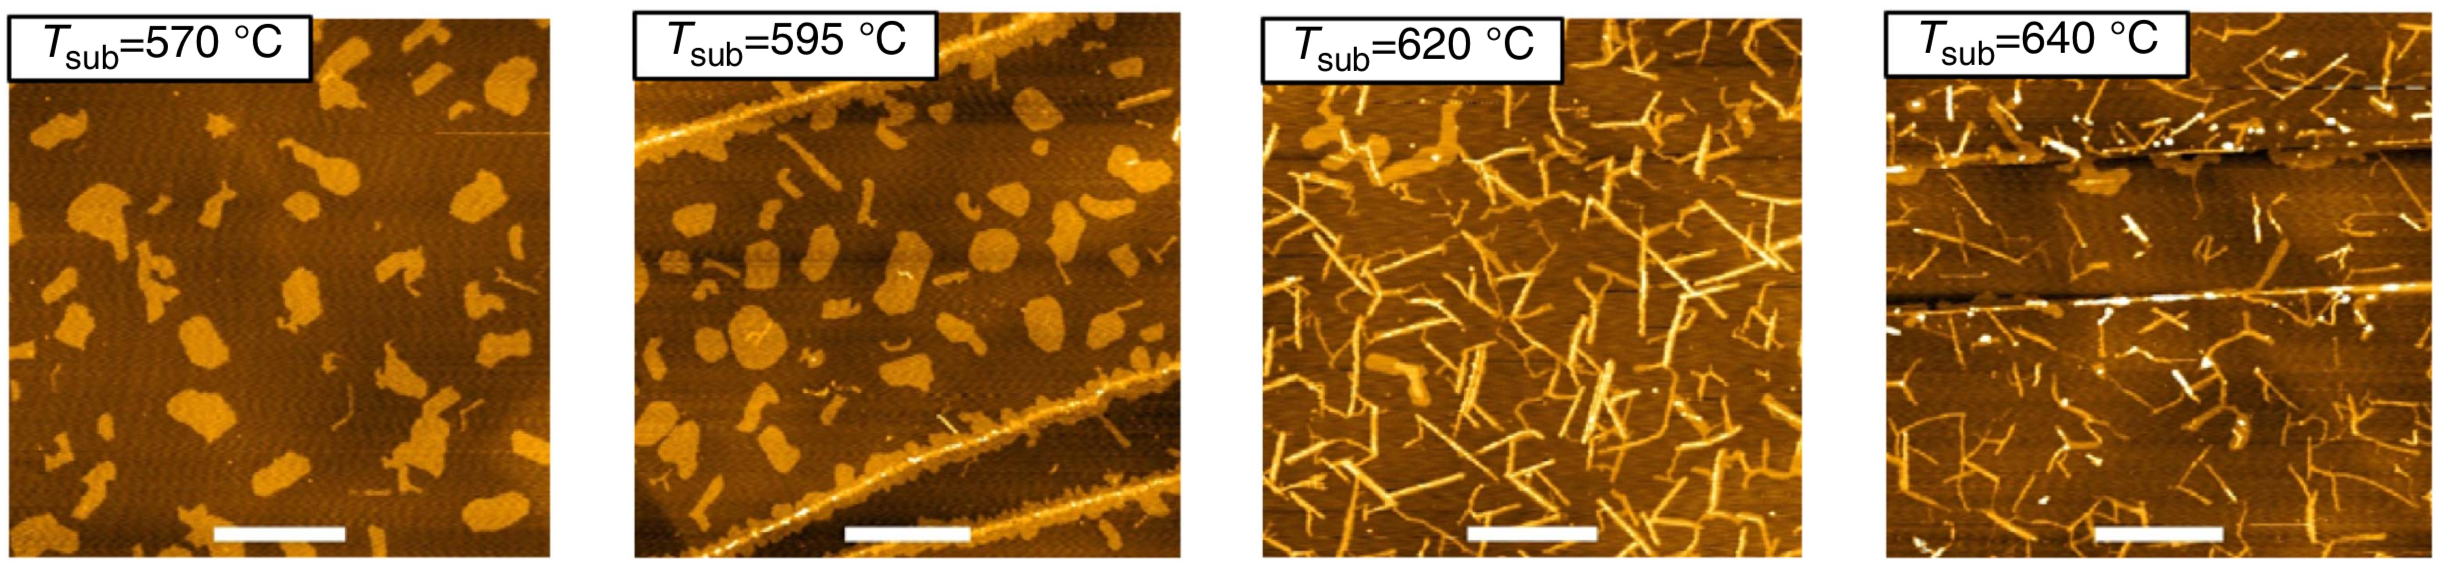
\includegraphics[scale = 0.35]{Introduction/nanoribbons}
\caption[Fabrication of \ac{TMD} nanoribbons]{Fabrication of \ac{TMD} nanoribbons. From left to right, we see \ac{AFM} images showing the appeareance of nanostructures ranging from \ac{2D} nanoislands to nanoribbons, as the temperature of the substrate is increased. The nanoribbons are grown by taking advantage of the temperature dependence of shape transformations occuring during the nonequilibrium growth of this kind of surface-based nanostructures. (taken from \cite{chen_fabrication_2017})}
\label{fig:fabrication}
\end{figure}
   
A high density of low-energy electronic states is localized at the zigzag edges, decaying quickly in the bulk, which suggests the possibility of magnetic ordering.
In fact, a mean field solution of the Hubbard model for a graphene nanoribbon shows that magnetic moments are localized at the edges \cite{yazyev_emergence_2010} (Figure \ref{fig:nanoribbons}, right).
QMC has been used to investigate edge-state magnetism beyond mean field in graphene \cite{feldner_dynamical_2011, golor_quantum_2013, cheng_strain-induced_2015, raczkowski_interplay_2017, yang_strain-tuning_2017}.
However, edge magnetism in TMD nanoribbons remains unexplored \cite{davelou_nanoribbon_2017}.
 
\begin{figure}[H]
\hspace{2cm}
\begin{minipage}[c]{0.1\textwidth}
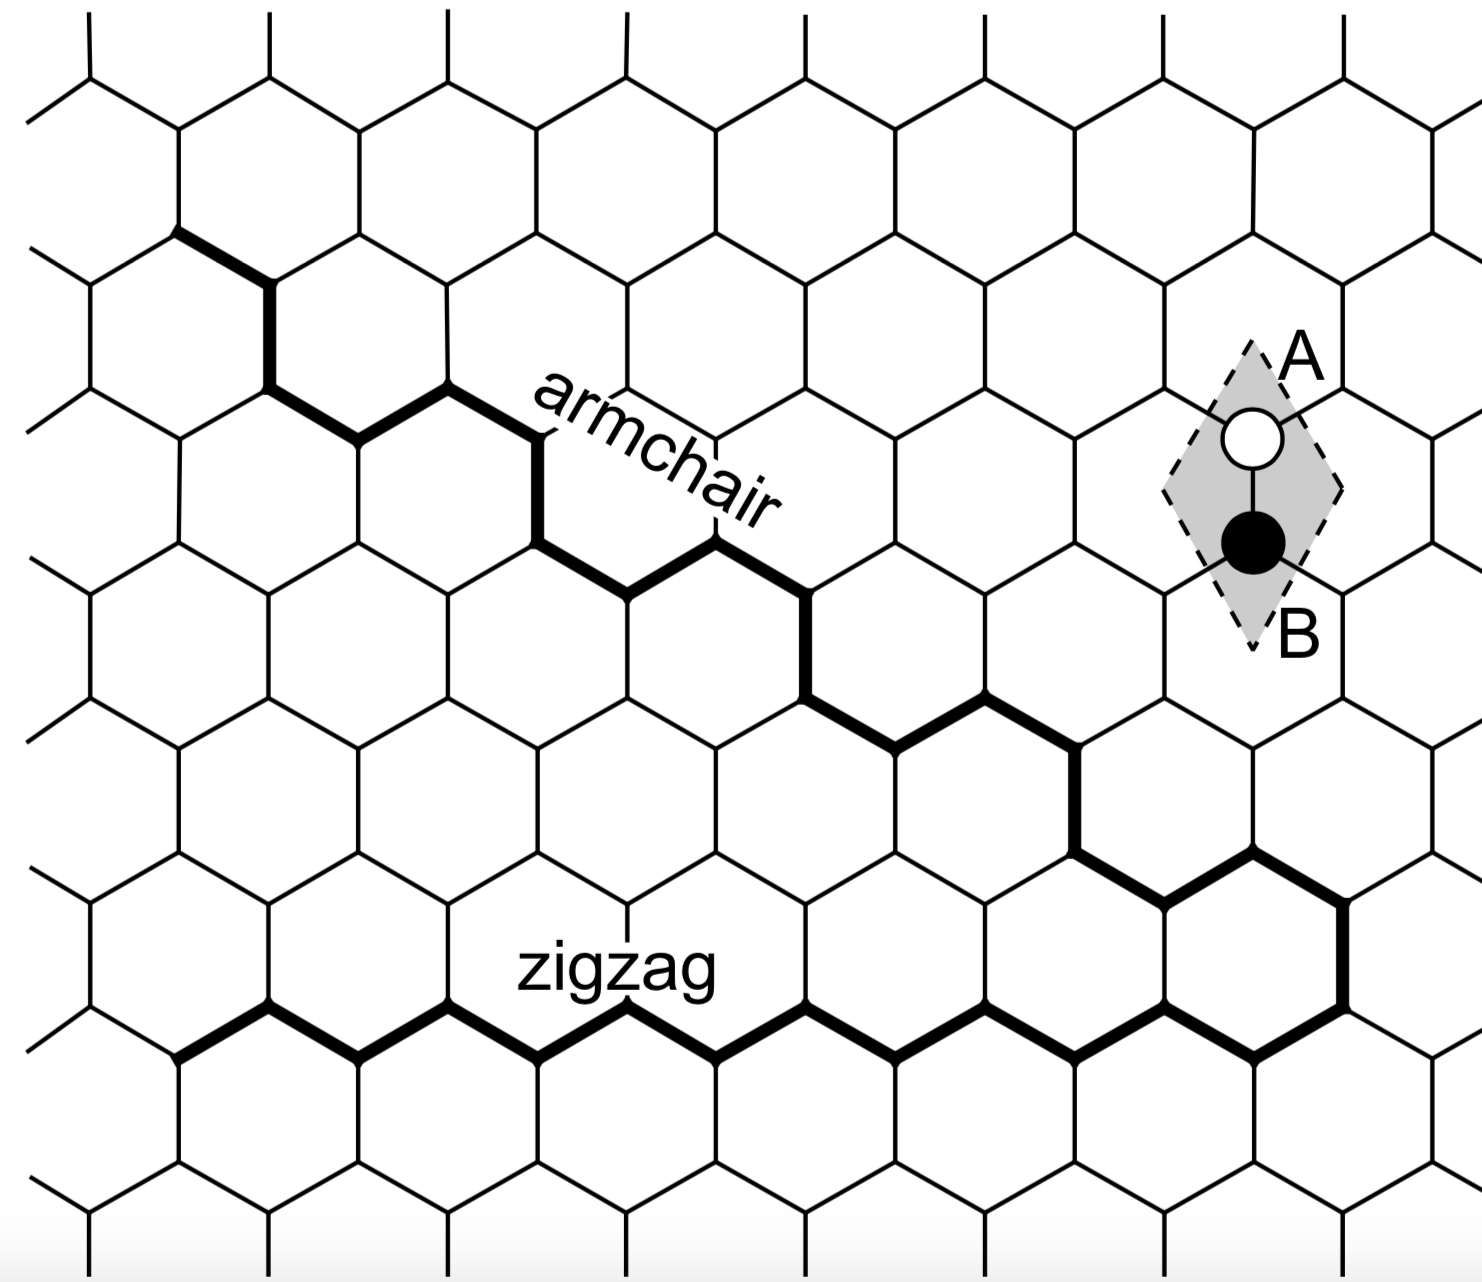
\includegraphics[scale = 0.22]{Introduction/zigzag}
\end{minipage} \hspace{6cm}
\begin{minipage}[c]{0.1\textwidth}
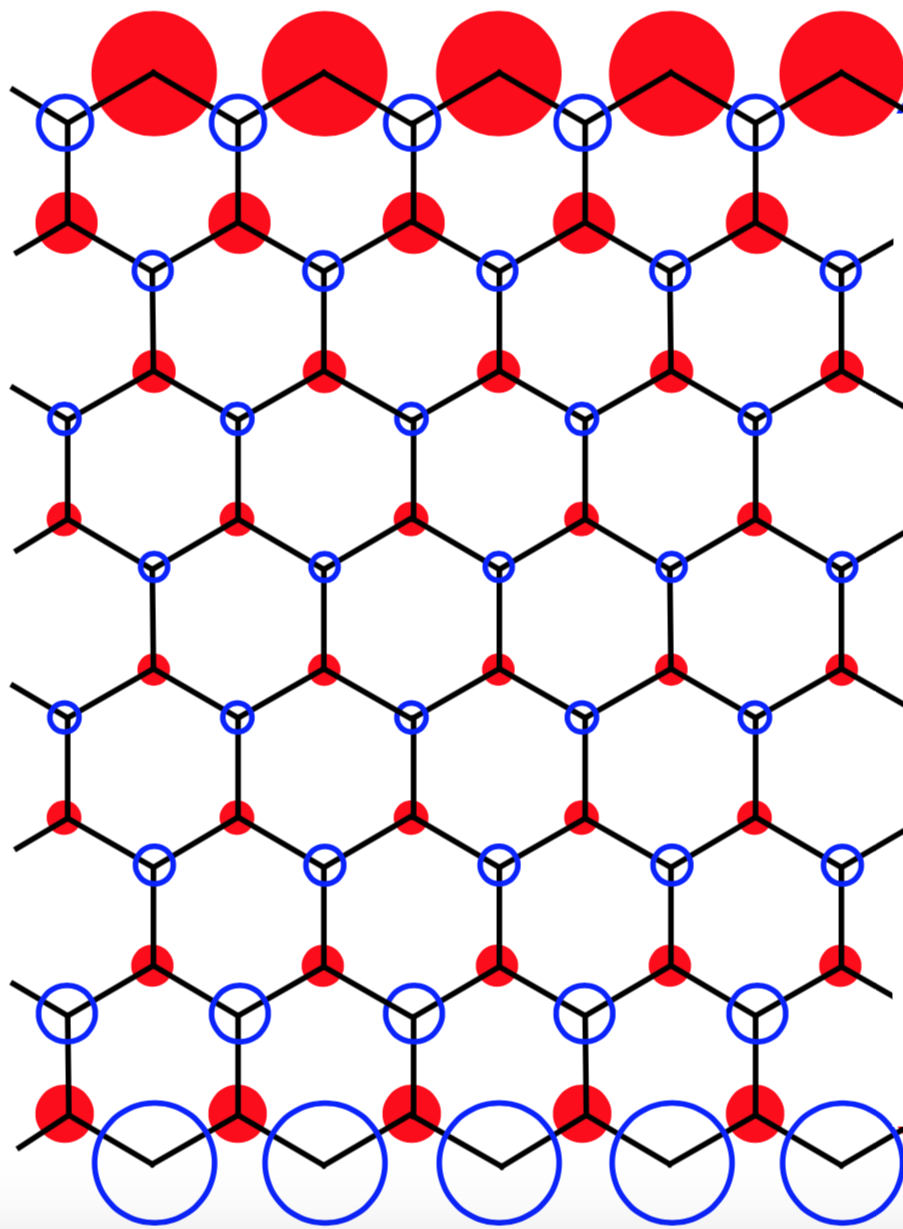
\includegraphics[scale = 0.23]{Introduction/edge_states}
\end{minipage}
 \caption[Zigzag edges of a nanoribbon and magnetism.]{Left: Two possible terminations of a \ac{TMD} nanoribbon condensing in a honeycomb lattice. Right: Local magnetic moments exist on the zig zag edges. The area of the circles corresponds to the magnitude of the magnetic moment, while the color red corresponds to a spin up density, and blue to a spin down density. The accumulation of electronic edge states leads to an \ac{AF} ground state (opposite edges with opposite magnetic moment). (taken from \cite{yazyev_emergence_2010}) \label{fig:nanoribbons}}
\end{figure}

While the zigzag graphene nanoribbon antiferromagnetic ground state is semiconducting, a state with interedge ferromagnetic orientation is a metal.
An example of an application based on the switching between the two states is a magnetorresistive sensor.
This device allows switching between low and high-resistance configurations, corresponding, respectively, to parallel, and antiparallel configurations of ferromagnetic leads at the ends of a nanoribbon.
An important application of this project is precisely the investigation of the possibility of edge-state magnetism, as is observed in graphene nanoribbons, for TMD nanoribbons, which could yield similarly innovative applications.


\subsection{Introduction to \acl{QMC}}

In principle, the properties of a quantum many-fermion system can all be deduced by solving an extremely complicated Schr\"odinger equation that takes into account the coupling of all (identical) particles of the system.
However, for the majority of systems the resulting integrals have no analytic solution, so we solve the problem by numerical integration.
But there is a myriad of methods to evaluate integrals numerically.
How do we pick the best one for this case? 
Multi-dimensional integrals are plagued by the curse of dimensionality.
Although the Newton-Cotes quadrature formulas (including, for example the Newton method, and Simpson's rules), Gaussian quadrature formulas, or Romberg's method all scale polynomially with the number of integration points, they become impractical as the dimension increases.
To use them, one would invoke Fubini's theorem to reduce the multi-dimensional integral to a series of one-dimensional integrals.
However, the number of function evaluations required to compute the whole integral grows exponentially with its dimension.
Monte Carlo methods preserve the polynomial scaling, thus yielding comparable accuracy with far less function evaluations. It is natural to use them since typically the state space of our quantum system is huge, leading to high dimensional integrals.

The Monte Carlo method is ubiquitous.
Its central idea is to use randomness to produce accurate estimates of deterministic integrals.
The term was coined by Nicolas Metropolis in 1949, first appearing in a seminal paper, in which it was described as a \say{statistical approach to the study of differential equations, or more generally, of integro-differential equations that occur in various branches of sciences}\cite{metropolis_monte_1949}.
Although it was used as early as 1777 in an experiment known as Buffon's needle - where one obtains an estimate of the constant $\pi$ by repeatedly throwing a needle randomly onto a sheet of paper with evenly spaced lines - it was crucially developed in the Los Alamos National Laboratory during World War II where the development of the first atomic bomb was completed, the primary objective of the Manhattan Project.
The method is particularly useful when one wants to sample from a probability distribution in an exponentially large state space.
In fact, it can in principle be used to solve any problem allowing a probabilistic formulation.

A variety of \acf{QMC} methods exists, using a sampling scheme based on the Metropolis algorithm, and variations thereof.
Variational and Diffusion \ac{QMC} are the simplest \ac{QMC} methods that allow one to capture some properties of correlated systems.
Although they already contain the main concepts used in this type of simulations, it is not always possible to use them. 
We will discuss their flaws and show how further refinement leads to the determinant, or auxiliary field method we ultimately used.

Using the Monte Carlo approach to study a many-fermion system implies overcoming a significant obstacle common to all \ac{QMC} methods - the so called \emph{fermion-sign problem}.
Pauli's exclusion principle implies that the many-fermion wave function is anti-symmetric, which leads to a sign oscillation that greatly impedes the accurate evaluation of averages of quantum observables.
The anti-symmetry constraint implies that a  straightforward weight interpretation of the wave function is not possible.
In the case of the finite temperature algorithm, the cancellations that occur when computing the average of any physical observable lead to poor statistical properties of the corresponding estimators.
This means that a massive amount of samples requiring enormous computer time are needed to obtain meaningful results.
In the case of the zero temperature algorithms, the situation is even worse.
It might not even be possible to design a stochastic process carrying the system to its ground state, as normally is done in \say{projective} methods\footnote{Methods that iteratively project a trial wave function onto the ground state.}: the wave function that is used as an initial proposal turns out to converge to a bosonic one, and the fermionic character of the system is lost.

As was proven by Troyer, the \emph{fermion-sign problem} has NP\footnote{NP or nondeterministic polynomial time, meaning that one can devise an algorithm that verifies the "yes" answer to a decision problem in polynomial time in the system size.
Note that the class $P$ - of polynomial time algorithms - is a subclass of NP.} computational complexity \cite{troyer_computational_2005}.
One of the greatest open questions in computer science is whether $P = NP$.
Solving the \emph{fermion-sign problem} would imply finding a solution to $P = NP$, which would constitute a major breakthrough.

\subsection{Monte Carlo Method in  Classical Statistical Physics}

Monte Carlo methods form the largest and arguably most useful class of numerical methods used to approach statistical physics problems.
Statistical physics often deals with computing quantities that describe the behavior of condensed matter systems.
The main difficulty one faces when doing so has to do with the collective nature of these systems.
Many identical components comprise these systems, and while the equations that govern the behavior of the whole may be easy to write down, their solution is in general a remarkably laborious mathematical problem.

The exponentially large number of configurations of a typical condensed matter system can be daunting.
Analytical solutions are more often than not hopeless and even numerical solutions are seemingly challenging.
However, they give valuable information lying between theory and experiment, and connecting them.

Suppose you try to sample uniformly from the probability distribution of all possible configurations of one of the aforementioned systems.
Changes are your algorithm will not end before the Universe does.
This is the computational complexity hurdle.
A related issue is that of finite size effects.
We are far from being able to simulate a macroscopically sized system. 
At best we can simulate a system that has only a minuscule fraction of the actual size of the corresponding real world system.
Amazingly there are techniques that allow us to efficiently extract information out of relatively small size simulations.
Nonetheless, increasing the system size systematically improves the reliability of a simulation.
Thus, the more efficient the algorithm is, the larger the system we can simulate in a fixed time.

The sheer number of equations describing a condensed matter system, and sometimes the strong coupling between them deems the task of finding an exact solution either very tough or even impossible.
It is not even clear whether an analytical solution would be of any use in many cases, and a statistical and numerical treatment often allows us to study more effectively the key properties of a system.

Strikingly, we are able to describe a system that is governed by a macroscopically large number of equations in terms of only a few variables.
The loss of information in doing so is only apparent.
The statistical description is so effective because most of the possible states of the system are extremely improbable when compared to the relevant very narrow part of configuration space.
The success of the field is largely attributed to the averaging out that naturally occurs when we measured a property of a macroscopic system.

The law of large numbers affords an approximation to integrals which can be written as an expectation of a random variable. Upon drawing enough independent samples from the corresponding distribution, the sample mean gets arbitrarily close to the integral at stake.

\begin{equation}\label{eq:int_mean}
\mathbb{E} [f(X)] = \int dx f(x) p(x),
\end{equation}
where $p(x)$ is the distribution of $X$. 

We could simply draw $M$ independent and identically distributed samples $x_{1,...M}$ from $p(x)$ and approximate the integral as

\begin{equation}
\frac{1}{M} \sum_{k=1}^M f (x_k) , 
\end{equation}
which in most cases converges to the desired expectation, as long as $M$ is large enough. How large?

\begin{equation}\label{eq:variance}
\text{Var}\bigg( \frac{1}{M} \sum_{k=1}^M f(x_k) \bigg) = \frac{1}{M} \text{Var}\bigg( f(x_1) \bigg) \sim \mathcal{O}\bigg(\frac{1}{M}\bigg)
\end{equation}

Thus, the correction to the sample mean is of order $\mathcal{O}(\frac{1}{\sqrt{M}})$ as long as $\text{Var}\big( f(x_1) \big) \sim 1$.

How do we sample from an arbitrary distribution $p(X)$? The idea is to first make an educated choice of a Markov Chain with the prescribed stationary distribution from which we ultimately desire to sample from, $p(X)$. After a sufficiently high number of steps, a Markov Chain Monte Carlo (MCMC) algorithm generates samples from the target distribution. Imposing some conditions on this Markov Chain, namely that it should be irreducible, aperiodic and positive recurrent, the ergodic theorem guarantees that the empirical measures of the aforementioned sampler approach the target stationary distribution. Another important condition to impose on this Markov Chain is detailed balance. Let the transition matrix be $\bm P = [P_{\mu \rightarrow \nu}]$, and the state space $\Omega$ be $\{\pi_\mu | \mu=1, ..., |\Omega| \}$, where $|\Omega|$ is the total number of possible states. Then, the condition of detailed balance is defined for all $\mu, \nu$ as

\begin{equation}\label{eq:detBal}
\pi_\mu P_{\mu \rightarrow \nu} = P_{\nu \rightarrow \mu} \pi_\nu
\end{equation}

Consider a system in state $\mu$ that makes transitions to state $\nu$ at a rate $R_{\mu \rightarrow  \nu}$ (that specifies the system's dynamics) and vice-versa.
The probability that a system is in state $\mu$ at time $t$, $p_\mu (t)$, such that $\sum_\mu p_\mu (t) = 1$, is given by the master equation(s):

\begin{equation}\label{eq:master}
\frac{d p_\mu}{dt} = \sum_\nu \big[ p_\nu (t) R_{\nu \rightarrow \mu} - p_\mu (t) R_{\mu \rightarrow \nu} \big] \quad \forall \mu \in \Omega
\end{equation}

The equilibrium occupation probabilities at finite temperature $T$ follow the Boltzmann distribution.

\begin{equation}
\pi_\mu = \lim_{t \rightarrow \infty} p_\mu (t) = \frac{1}{Z} e^{ - E_\mu / k_B T} ,
\end{equation}
where $E_\mu$ is the energy of state $\mu$, $k_B$ is Boltzmann's constant, and $Z$ is the partition function, from which we can extract thermodynamic functions in terms of expectations of physical quantities $\left\langle Q \right\rangle$, and response functions in terms of their variance $\sigma_Q^{\,\, 2}$.

Imposing the condition of stationarity on equation (\ref{eq:master}), $d_t p_\mu = 0$ , and noting that $ P_{\mu\rightarrow \nu} = R_{\mu\rightarrow \nu}  dt$, we obtain the equilibrium condition

\begin{equation}\label{eq:equilibrium}
\sum_\nu \pi_\mu P_{\mu \rightarrow \nu} = \sum_\nu P_{\nu \rightarrow \mu} \pi_\nu \iff \pi_\mu \sum_\nu P_{\mu \rightarrow \nu} = \sum_\nu P_{\nu \rightarrow \mu} \pi_\nu \iff \pi_\mu = \sum_\nu P_{\nu \rightarrow \mu} \pi_\nu
\end{equation}

This condition is enough to ensure convergence to an equilibrium of the dynamics of the Markov process.
However, it does not guarantee that the reached distribution is our desired one, $\bm \pi$, after running the process for long enough.
The probability of a state evolves according to

\begin{equation}
\pi_\nu ( t + 1 ) = \sum_\mu P_{\mu\rightarrow\nu}  \pi_\mu ( t ) \iff \bm \pi ( t + 1 ) = \bm P \bm \pi ( t )
\end{equation}

The stationary distribution of a Markov chain obeys

\begin{equation}
\bm \pi ( \infty ) = \bm P \bm \pi ( \infty ) ,
\end{equation}
however, condition (\ref{eq:equilibrium}) also allows  for limit cycles of length $n$, where $\bm \pi$ rotates around a number of configurations:

\begin{equation}
\bm \pi ( \infty ) = \bm P^n \bm \pi ( \infty ) ,
\end{equation}
where $\bm P^n$ is the n-th power of $\bm P$.

Detailed balance is a stronger requirement than the equilibrium condition, which eliminates limit cycles, thus ensuring that our sampler draws configurations from the desired distribution.
Intuitively, detailed balance corresponds to incorporating time-reversal symmetry in a simulation.
The condition imposes a constraint on the Markov transition probabilities:

\begin{equation}\label{eq:markovCondition}
\frac{P_{\mu\rightarrow\nu}}{P_{\nu\rightarrow\mu}} = \frac{\pi_\nu}{\pi_\mu} = e^{-\beta ( E_\nu - E_\mu ) }
\end{equation}

Crucially, Monte Carlo methods employ \emph{importance sampling}.
It turns out that we can improve upon our estimate of $\mathbb{E} [f(X)]$ by introducing a separate distribution $q(x)$, and defining the weight function as $w(x) = p(x)/ q(x)$.
Then, we can rewrite equation (\ref{eq:int_mean}):

\begin{equation}
\mathbb{E} [f(X)] = \int dx f(x) q(x) w(x) = \mathbb{E} [f(Y) w(Y)],
\end{equation}
with $Y \sim q$, i.e. the random variable $Y$ follows the distribution $q(Y)$.

It appears as though we didn't gain anything. However, by choosing $q$ wisely, we can actually reduce the variance we computed in equation (\ref{eq:variance}):

\begin{equation}
\text{Var}\bigg( \frac{1}{M} \sum_{k=1}^M f(y_k) w(y_k) \bigg) = \frac{1}{M} \text{Var}\bigg( f(y_1) w(y_1) \bigg)
\end{equation}

Since we didn't make any assumptions about $q(Y)$, it may be chosen so as to minimize the variance, hence the error of the Monte Carlo estimator, improving the approximation of the expectation. However, note that the error remains proportional to $\frac{1}{\sqrt{M}}$.
In practice, we devise a method to select the portion of state space which contains states contributing more significantly to the average.
This procedure ensures that $\text{Var}\big( f(y_1) w(y_1) \big) \sim 1$, improving the efficiency of our sampler.
The choice of the weight function translates to the averaging process by changing the estimator.
Explicitly computing the average

\begin{equation}
\left\langle Q \right\rangle = \frac{ \sum_\mu Q_\mu e^{-\beta E_\mu} }{ \sum_\mu e^{-\beta E_\mu}}
\end{equation}
is only tractable for very small systems.
In practice, we choose a subset of M states $\{\mu_1, \mu_2, ..., \mu_M \} $, and estimate the average as

\begin{equation}
Q_M = \frac{ \sum_{i=1}^M Q_{\mu_i} \pi_{\mu_i}^{-1} e^{ -\beta E_{\mu_i} } }{ \sum_{j=1}^M \pi_{\mu_j}^{-1} e^{ -\beta E_{\mu_j} }  }
\end{equation}

The estimate improves as $N$ increases, and when $N\rightarrow \infty$, $Q_M \rightarrow \left\langle Q \right\rangle$.
The accuracy of the estimator depends on the choice of the probabilities $\bm \pi$, which is related to the aforementioned variance.
For example, if $\bm \pi$ corresponds to the uniform distribution, i.e. $\pi_\mu = \frac{1}{| \Omega |} \forall \mu \in \Omega$, we have

\begin{equation}
Q_M = \frac{ \sum_{i=1}^M Q_{\mu_i} e^{ -\beta E_{\mu_i} } }{ \sum_{j=1}^M e^{ -\beta E_{\mu_j} }  } ,
\end{equation}
which turns out to be a poor choice since most of the visited states contribute negligibly to the average, leading to an inaccurate estimate.
The sum is dominated by a small subset of states, which we would like to access.
The idea of the Quantum (Classical) Monte Carlo method is to simulate the random quantum (thermal) fluctuations of a system, as it oscillates between states in a given time frame \cite{newman_monte_1999}. Instead of visiting these states uniformly, the most relevant part of the phase space is sampled more frequently, overcoming the seemingly exponential complexity of computing a sample mean numerically.
Even though only a small fraction of the system's states are sampled, we then obtain an accurate estimate of physical quantities of interest, namely energy, and correlation functions. This is implemented via a proposal-acceptance scheme.

To exploit the freedom given by condition (\ref{eq:markovCondition}), we note that we can always introduce a non-zero \say{stay-at-home} probability $P_{\mu \rightarrow \mu} \in [0, 1] $.
Regardless of its value, detailed balance is satisfied.
Similarly, any adjustment in $P_{\mu\rightarrow \nu}$ must be compensated by changing $P_{\nu\rightarrow \mu}$ to preserve their ratio.
Break the transition probability into a selection probability and an acceptance ratio, respectively:

\begin{equation}
\frac{P_{\mu\rightarrow\nu}}{P_{\nu\rightarrow\mu}}= \frac{G_{ \mu\rightarrow\nu} A_{\mu\rightarrow\nu}}{G_{ \nu\rightarrow\mu} A_{\nu\rightarrow\mu}}
\end{equation}

The Markov process now consists of generating a chain of states according to $G_{ \mu\rightarrow\nu}$, which are then accepted or rejected depending on $A_{\mu\rightarrow\nu}$.
Since we want to make the algorithm as efficient as possible, we want to make the acceptance ratio as close to one as possible to avoid useless steps.	
The most common way to do this is to fix the largest of them to one, and ajust the other accordingly.
The acceptance ratio will be close to one more often if $G_{ \mu\rightarrow\nu}$ includes most of the dependence of $P_{\mu\rightarrow\nu}$ on the characteristics of the states $\mu, \nu$.
Ideally, states would always be selected with the correct transition probability, and the acceptance ratio would be fixed to unity.
Good algorithms approach this situation, and much effort has been directed at optimizing them to do so.

By far, the most common sampling scheme choice is the Metropolis-Hastings algorithm, which we now  describe.

We select the transition probability to be uniform, and impose detailed balance through the choice of the acceptance ratios:

\begin{equation}
\frac{ P_{\mu\rightarrow\nu }}{ P_{\nu\rightarrow\mu }} = \frac{ A_{\mu\rightarrow\nu }}{ A_{\nu\rightarrow\mu } } = e^{-\beta ( E_\nu - E_\mu )}
\end{equation}

Suppose that $E_\mu < E_\nu $.
Then, $A ( \nu \rightarrow \mu ) > A ( \mu \rightarrow \nu ) $, and since only the acceptance ratio is fixed, we may freely set $A ( \nu \rightarrow \mu ) = 1$, which fixes $A ( \mu \rightarrow \nu ) = e^{-\beta ( E_\nu - E_\mu ) }$.
This choice maximizes the efficiency of the algorithm.
In short, we propose a random new state uniformly, and then we accept it with probability $A_{\mu\rightarrow \nu} = \min (1,  e^{-\beta ( E_\nu - E_\mu )})$.

Before we can use the states generated by our sampler to measure averages of physical quantities, we must reach the stationary distribution of the Markov process.
We consider this condition to be satisfied after a time $\tau_{\text{eq}}$, measured in steps of the algorithm.
When we consider a lattice model with a discrete set of states at each site $i = 1, 2, ..., N$, we say that a \emph{sweep} is completed whenever $N$ Monte Carlo steps are performed.
Thus, the number of \say{warm-up} sweeps is $W = \tau_{\text{eq}} / N$.

Before running a simulation, we need to decide how many sweeps we need to get an accurate estimate of the average.
The problem is that we need uncorrelated samples to average over.
To clarify, let us choose a specific model.
The paradigmatic model of statistical physics is the Ising model, a classical model of a magnet, which consists of considering spins-$1/2$ on a lattice, interacting only with their nearest neighbors.
Since each spin can only take on two values, say $\pm 1$, there are $2^N$ possible states.
The Hamiltonian reads

\begin{equation}
H = - J \sum_{\left\langle i, j \right\rangle } s_i s_j - B \sum_i s_i ,
\end{equation}
where $\left\langle i, j \right\rangle$ means that $i, j $ are nearest neighbors on the lattice.

A simple strategy to sample configurations of the Ising model is single-spin-flip dynamics.
We start with a random configuration of the spins, and then propose new configurations at each step by flipping a single spin at a given site.
A sweep is completed after we propose a spin flip at every site on the lattice.

Consecutive configurations generated by this chain differ only slightly.
Thus, it takes some time for the system to reach a configuration which is significantly different from the initial one.
This characteristic time is called the correlation time $\tau_c$.
A rigorous manner to estimate $\tau_c$ is through the time-displaced auto-correlation function associated to some quantity being measured.
An example of a relevant quantity for the case of the Ising model is the magnetization per site:

\begin{equation}
m = \frac{1}{N} \sum_i s_i
\end{equation}

Its associated time-displaced auto-correlation is

\begin{equation}
\chi_m ( t ) = \int dt' \bigg( m ( t' ) - \left\langle m \right\rangle \bigg) \bigg( m ( t' + t ) - \left\langle m \right\rangle \bigg) = \int dt' \bigg( m ( t' ) m ( t' + t ) - \left\langle m \right\rangle^2 \bigg)
\end{equation}
giving a measure of how correlated two measurements of the magnetization separated by a simulation time $t$ are.

The typical time-scale on which $\chi_m (t)$ falls off is a measure of the correlation time of the simulation.
In particular, at long times it falls off exponentially.
The definition of $\tau_c$ stems from this characteristic long-time behavior: $\chi_m (t) \sim e^{-t / \tau_c}$.
In practice, after waiting for $2\tau_c$, the measurements are virtually uncorrelated.
Let $A$ be the number of sweeps roughly  corresponding to $2\tau_c$ steps.
Then, if we make $S$ sweeps of the lattice during the simulation, the number of measurements (waiting for $A$ sweeps between them) is

\begin{equation}
M = \frac{S - W}{A}
\end{equation}

There are many ways to estimate $\tau_c$ from $\chi_m (t)$.
The simplest consists of making an exponential fit in a given range of times.
However, this might be unreliable since the estimate depends strongly on the chosen range.
An alternative is to compute the \say{integrated} correlation time:

\begin{equation}
\int_0^\infty dt \frac{\chi_m ( t ) }{\chi_m ( 0 ) } = \int_0^\infty dt e^{-t / \tau_c} = \tau_c  ,
\end{equation}
which is less sensitive, but not perfect either since the error that is introduced when the assumption  that \say{long-time} behavior has been reached is arbitrary and introduces an uncontrolled error.
Moreover, the very long-time behavior of the auto-correlation is rather noisy and must be excluded.

Using measured data for the magnetization at evenly-spaced times, we may construct the time-displaced auto-correlation function up to an unimportant constant, which does not affect the estimate of the correlation time:

\begin{equation}
\chi_m (t) = \frac{1}{ t_{\text{max}} - t } \sum_{t' = 0}^{t_{\text{max}} - t } m (t') m(t' + t) - \frac{1}{ t_{\text{max}} - t } \sum_{t' = 0}^{t_{\text{max}} - t } m (t') \frac{1}{ t_{\text{max}} - t } \sum_{t' = 0}^{t_{\text{max}} - t } m(t' + t) ,
\end{equation}
where $t_{\text{max}}$ is the total simulation time.

One should be careful when using this expression at very long times.
As $t$ approaches $t_{\text{max}}$, the upper limit of the sums decreases, and the integration interval becomes narrower.
Since $m (t)$ fluctuates randomly at very long times, the statistical error associated to $\chi_m (t)$ becomes more prominent as $t$ approaches $t_{\text{max}}$.
This turns out not to be problematic since typical simulations run for many correlation times.
Thus, the tails of the auto-correlation may safely be neglected because the correlations will have already vanished, by definition.

To finish our discussion on the issue of correlations, we note that if we have a total of $n_s$ samples of, for instance, magnetization data, the complexity of computing $\chi_m$ is $\mathcal{O}(n_s^2)$.
It is possible to speed up this process by computing its Fourier transform $\tilde{\chi}_m(\omega)$, and inverting to recover $\chi_m (t)$.
This can be done via a standard \ac{FFT} algorithm in $\mathcal{O}(2 n_s \log n_s )$ flops.
To do this, we apply the following trick

\begin{equation}
\begin{split}
\tilde{\chi}_m ( \omega ) &= \int dt e^{i\omega t} \int dt' \bigg( m ( t' ) - \left\langle m \right\rangle \bigg) \bigg( m ( t' + t ) - \left\langle m \right\rangle \bigg) \\
&= \int dt \int dt' e^{-i\omega t'} \bigg( m ( t' ) - \left\langle m \right\rangle \bigg) e^{i\omega ( t' + t )} \bigg( m ( t' + t ) - \left\langle m \right\rangle \bigg) \\
&= \tilde{m}' (\omega) \tilde{m}' (- \omega) = | \tilde{m}' (\omega) |^2 ,
\end{split} 
\end{equation}
where $\tilde{m}' (\omega)$ is the Fourier transform of $m' (t) = m(t) - \left\langle m \right\rangle$\footnote{The only difference between $\tilde{m}' (\omega)$ and $\tilde{m} (\omega)$, is that $\tilde{m}' (0) = 0$, while $\tilde{m} (0) \neq 0$. Thus, one can also compute $\tilde{m} (\omega)$ and then set its $\omega = 0$ component to zero.}.

\subsection{Variational Monte Carlo}

Variational techniques rely on an educated guess for the wave function of the system.
One introduces a set of variational parameters $\bm \alpha$ that are then tuned according to a variational principle.
Then, we may use the optimized trial wave function to compute physical quantities of interest using Monte Carlo.
The method is used to obtain zero temperature properties of a given model.
Note that it requires prior knowledge about the system to propose an approximate wave function in the first place.

A particularly relevant observable is the variational energy $E_V$ associated to a trial ground state.
Let $\bm r$ be the $3N$ spatial coordinates of the $N$ electrons.
Given the Hamiltonian of the system $\mathcal{H}$, and a trial wave function $\psi (\bm r)$ - a guess of the wave function representing the ground state - one can compute the corresponding variational energy.

\begin{equation}\label{eq:variational_energy}
E_V = \frac{\left\langle \psi | \mathcal{H} | \psi \right \rangle}{\left\langle \psi | \psi \right \rangle} = \frac{ \int d\bm r |\psi (\bm r)|^2 E_L (\bm r)}{\int d\bm r | \psi (\bm r)|^2 } = \int d\bm r\rho (\bm r) E_L (\bm r) ,
\end{equation}
where the local energy $E_L (\bm r)$ is defined as

\begin{equation}\label{eq:local_energy}
E_L = \frac{\mathcal{H} \psi (\bm r) }{\psi (\bm r)}
\end{equation}
and the probability distribution $\rho (\bm r)$ is defined as

\begin{equation}\label{eq:rho}
\rho (\bm r) = \frac{ | \psi (\bm r) |^2}{ \int d\bm r' | \psi (\bm r') |^2}
\end{equation}

Note that we managed to recast the variational energy as an average of the \emph{local} energy, $\left\langle E_L \right\rangle $, over the the distribution $\rho$.
This may be computed using the Monte Carlo method by sampling $M$ points $\bm r_k$ from distribution $\rho (\bm r)$:

\begin{equation}\label{eq:average}
E_V \approx \overline{E}_L = \frac{1}{M} \sum_{k= 1}^{M} E_L (\bm r_k) ,
\end{equation}
where $\overline {X}$ denotes a sample mean of the random variable $X$.

Let the ground state energy be $E_0$.
Then, states are optimized according to the variational principle:

\begin{equation}
E_V(\bm \alpha) = \frac{\left\langle \psi_{\bm \alpha} | \mathcal{H} | \psi_{\bm \alpha} \right\rangle}{\left\langle\psi_{\bm \alpha} | \psi_{\bm \alpha} \right\rangle} \ge E_0,
\end{equation}
where $\psi_{\bm \alpha}$ is the trial ground state wave function for the set of variational parameters ${\bm \alpha}$.

By varying $\bm \alpha$ we aim to obtain a variational energy that is as close as possible to the true ground state energy.
Since $E_V(\bm \alpha)$ is bounded from below, this is equivalent to minimizing it in the hope that $E_V(\bm \alpha_{min}) \gtrsim E_0$, i.e. the bound is tight.

The finite sampling size $M$, of course, introduces a statistical error common to all Monte Carlo methods. 
However, the use of an approximate wave function introduces a systematic error that is hard to control since trial wave functions are generally introduced based on approximate, or heuristic arguments.

\subsection{Diffusion Monte Carlo}\label{subsec:dmc}

Variational Monte Carlo is severely limited by the use of a trial wave function $\psi_{\bm \alpha} (\bm r)$ because we may even not have enough information to even construct a reliable variational wave function.

Diffusion \ac{QMC} allows the simulation of a many-body system while having only a limited knowledge of the system's physical properties.
While it is exact for many-boson systems, it is only approximate for many-fermion systems.
The idea is to map the Schr\"odinger equation into  an imaginary-time diffusion equation.
Excited states are then filtered out by a diffusion process as we advance in imaginary-time.
In imaginary-time $\tau = - i t$, the solution to the Schr\"odinger equation in terms of a formal series expansion in the eigenfunctions of the hamiltonian becomes a series of transients $e^{-E_n \tau}, \, n \in \mathbb{N}$.
The longest lasting of these is the ground state  \cite{kosztin_introduction_1996}.

The idea of the diffusion method is to generate samples using the exact ground state wave function $\psi_0 (\bm r)$ \cite{toulouse_chapter_2016}.
The associated exact energy $E_0$ is the matrix element of the hamiltonian calculated using a trial wave function and the ground state wave function.

\begin{equation}
E_0 = \frac{ \left\langle \psi_0 |E_0 \mathbbm{1} | \psi \right\rangle}{\left\langle \psi_0 | \psi \right\rangle} = \frac{\left\langle \psi_0 | \mathcal{H} | \psi \right\rangle}{ \left\langle\psi_0 | \psi \right\rangle} = \frac{\int d\bm r \psi_0^\star (\bm r) \psi (\bm r) E_L (\bm r)}{\int d\bm r\psi_0^\star (\bm r) \psi (\bm r)}
\end{equation}

Note that using this trick we avoid the computation of $\mathcal{H} \psi_0 = E_0 \psi_0$, that is, the ground state energy.
Instead, we approximate the integral by considering $M$ configuration samples $\bm r_{k = 1,..., N}$ in a similar spirit to that of Variational \ac{QMC}.
Notice that the integral consists of a local energy of the trial wave function $E_L (\bm r) = \frac{\mathcal{H} \psi (\bm r)}{\psi (\bm r)}$ averaged over a mixed distribution from which we draw a sample of points $\bm r_{k=1,...M}$:

\begin{equation}
f(\bm r) = \frac{\psi_0^\star (\bm r) \psi (\bm r) }{ \int d\bm r  \psi_0 (\bm r) \psi (\bm r)}
\end{equation}

Although the method is, of course, aimed at probing many-body systems, let us consider a single particle in \acl{1D} for simplicity for illustrating the method.
Performing a Wick rotation - effectively going to imaginary time - and shifting the energy, the Schr\"odinger equation becomes

\begin{equation}
\frac{\partial \psi ( x, \tau )}{\partial\tau}  = -\frac{1}{2m}\frac{\partial^2 \psi ( x, \tau )}{\partial x^2} - \bigg[ V(x) - E_T \bigg] \psi( x, \tau ) 
\end{equation}

The exact ground state wave function $\psi_0 ( x )$ is obtained as the longest lasting transient state in imaginary time: we are interested in the asymptotic behavior of the series expansion constituting the formal solution of the Schr\"odinger equation

\begin{equation}
\psi (x, \tau) = \sum_{n=0}^{\infty} c_n \psi_n (x) e^{-(E_n - E_T)\tau}
\end{equation}

Imaginary time evolution is governed by

\begin{equation}\label{eq:im_ev}
\begin{split}
&\left| \psi (t) \right\rangle = \lim_{\tau \rightarrow \infty} \sum_i e^{-(E_i - E_T) \tau} \left|\psi_i \right\rangle \left\langle \psi_i | \psi \right\rangle = \\
&= \lim_{\tau \rightarrow \infty} e^{-(E_0 - E_T)\tau} \left| \psi_0 \right\rangle \left\langle \psi_0 | \psi \right\rangle 
\end{split}
\end{equation}


If $E_T > E_0$ the wave function diverges exponentially fast: $\lim_{\tau \rightarrow \infty} \psi ( x, \tau) = \infty$.
Similarly, for $E_T < E_0$ it vanishes exponentially fast: $\lim_{\tau \rightarrow \infty} \psi ( x, \tau) = 0$.
However, if $E_T = E_0$ the wave function converges to the ground state one up to a constant factor.

\begin{equation}\label{eq:dmc}
\lim_{\tau \rightarrow \infty} \psi ( x, \tau) = c_0 \psi_0 (x) \,\,\, \text{, or} \quad \lim_{\tau \rightarrow \infty} \left|\psi (\tau) \right\rangle \propto \left| \psi_0 \right\rangle
\end{equation}

Diffusion \ac{QMC} makes use of equation (\ref{eq:dmc}), approximating $\phi_0(x)$ by $\psi (x, \tau)$ for sufficiently long time.
The only requirement is that $\psi (x, \tau)$ and $\psi_0(x)$ overlap significantly so that $c_0$ is large enough to be numerically measurable, and we can always center a positive trial wave function in a region where $\psi_0(x)$ is large enough.
Of course, this is always possible for a single particle, but note that it might fail for a many-fermion system, for which the wave function crosses a number of nodes due to its anti-symmetric nature.